\documentclass[a4paper,10pt]{article}
\usepackage[utf8]{inputenc}
\usepackage{hyperref}
\usepackage{listings}
\usepackage{graphicx}
\usepackage{color}
\usepackage{multirow}

\newcommand{\tobetested}[0]{\colorbox{red}{\textbf{To Be Tested}}}
\newcommand{\tested}[0]{\colorbox{green}{\textbf{Working}}}

%opening
\title{Design considerations for embedded systems with sensing capabilities in urban areas}
\author{}

\begin{document}

\maketitle

\begin{abstract}
 The following document describes the design considerations when building an embedded system that has sensing capabilities and is to be deployment in an urban area.
\end{abstract}

\newpage

\tableofcontents

\newpage

\lstset{ %
%  backgroundcolor=\color{white},   % choose the background color; you must add \usepackage{color} or \usepackage{xcolor}
  basicstyle=\small\ttfamily,        % the size of the fonts that are used for the code
%  breakatwhitespace=false,         % sets if automatic breaks should only happen at whitespace
  breaklines=true,                 % sets automatic line breaking
  captionpos=t,                    % sets the caption-position to bottom
  commentstyle=\color{green},    % comment style
%  deletekeywords={...},            % if you want to delete keywords from the given language
  escapeinside={\%*}{*)},          % if you want to add LaTeX within your code
%  extendedchars=true,              % lets you use non-ASCII characters; for 8-bits encodings only, does not work with UTF-8
  frame=single,                    % adds a frame around the code
%  keepspaces=true,                 % keeps spaces in text, useful for keeping indentation of code (possibly needs columns=flexible)
%  keywordstyle=\color{blue},       % keyword style
%  language=Octave,                 % the language of the code
%  morekeywords={*,...},            % if you want to add more keywords to the set
  numbers=left,                    % where to put the line-numbers; possible values are (none, left, right)
  numbersep=5pt,                   % how far the line-numbers are from the code
  numberstyle=\tiny\color{red}, % the style that is used for the line-numbers
%  rulecolor=\color{black},         % if not set, the frame-color may be changed on line-breaks within not-black text (e.g. comments (green here))
%  showspaces=false,                % show spaces everywhere adding particular underscores; it overrides 'showstringspaces'
%  showstringspaces=false,          % underline spaces within strings only
%  showtabs=false,                  % show tabs within strings adding particular underscores
  stepnumber=1,                    % the step between two line-numbers. If it's 1, each line will be numbered
%  stringstyle=\color{mymauve},     % string literal style
%  tabsize=2,                       % sets default tabsize to 2 spaces
  title=\lstname                   % show the filename of files included with \lstinputlisting; also try caption instead of title
}


\section{Introduction}

small introduction on embedded systems.

previous work on fault tolerance and security

``Heat flux and wear-off (e.g. electro-migration) can cause functional units to stop working after some time either for the duration of certain environmental conditions, such as temperature being above a certain threshold, or forever'' [ Dieter K. Schroder. Negative bias temperature instability: What do we understand? Microelectronics Reliability , 47(6):841–852, 200]

Design and Architectures for Dependable Embedded Systems [http://spp1500.itec.kit.edu/]

\section{Privacy}

As mention earlier privacy becomes a first order considerations when deploying sensors on an urban environment. The reason for that is that as the sensors collect data, sensitive information about habitats or travelers around them may also be collected. This can happen accidentally or with a malicious intent. Following a list of possible sensors together with normal and abusive scenarios is gonna be presented.

The case of a wireless cards: a wireless card can act as an activity/traffic sensor. Metrics that can be recorded include traffic load, unique MAC addresses, possibly unique urls of unencrypted communication, or even keyword occurrence of unencrypted instant messaging. These information can be used to present an image of how communication heavy the area is, or how event news propagate from their source. However, miss-use can also happen and personal information can be extracted; like personal messages, preferences, or even walking routes and presence inside building.
  
The case of RFID readers: An RFID reader can be used for enabling some feature on the sensor or communication of the sensor and an application in an approaching device. In a malicious scenario the rfid reader can be used to extract information from rfid cards that come into its vicinity and otherwise have no correlation with the system (Ventra Cards, ID Cards, Credit Cards).
  
The case of image or video recording: image capturing can be used in conjunction with a figure recognition/tracking software to present information about the density of people or vehicles near the node. A possible miss-use would be face recognition for route tracking, presence verification, or even extraction of conversations.
  
The case of audio recording: audio recording can be used to collect information about noise levels or species identification in a location. Or it can be used to record conversations.
  
  
For the aforementioned reasons requirements about the operation and oversight of the sensors' data collection need to be specified.

\subsection{Operation Requirements}
Should we require some kind of key for a sensor to join the embedded system?


The embedded system should have control over what it senses all the time.
What is sensed should be public at all time and monitored so that in case of a privacy incident information leakage is minimized

Automatic isolation/lock of offending sensors.

Particularly intrusive sensors may need to be left out and alternatives should be considered.



\subsection{Oversight Requirements}

An independent, from the operational authority, observer should be able to have a full picture of what has been collected by the sensors and who has access to it in an easy manner.

\section{Security}

Security is the way to support the privacy requirements, maintain control over the system, and assure data integrity.

\subsection{Physical Access Control}

As it was initially stated a significant part of the infrastructure is gonna be in public places. Thus we need to provision against security threads due to physical access on these machines; control nodes, guest nodes, and sensors. The event of a device theft should be considered as certain.

Our goals are: node breach isolation, attack impairment, attack repel, equipment tracking.

\subsubsection{Isolation}

One of the most important requirement in the design process should be that the breach/theft of a single node could not jeopardize the security of the remaining system. Things that are affected by this requirement are the existence of plain-text passwords, key-pairs for automatic authentication and login, and encryption keys.

Ideally no key pair co-exists at any of the publicly available systems, an exception to that rule is the public-private pair that is unique to the machine.

The idea of full partition encryption should be considered. The benefits and disadvantages should be weighted. 

We need to find how to prevent someone with access to the data stored on a guest node or node controller to impersonate that node to gain access to the system.

\subsubsection{Impair attacks}

To deter or impair attacks a first step is to physically secure the system. Using a cable-padlock combination or an equivalent approach the chassis of the system should be locked to a fixed object. This will not stop the prepared thief  but would increase the necessary effort and time, improving the possibility of someone seeing and reporting the incident. The last remark presents another consideration which is how the location/placement of the system affects its security. A more secretive location may make it harder for a system to be found but when found provide cover to an attacker, whereas a more public location exposes the system but gives no cover to an attacker and increases the chance of a report from a bystander. A security improvement would be the replacement of common screws with non-standard screws (like Torx screws) \url{https://en.wikipedia.org/wiki/List_of_screw_drives}.
Except for trying to prevent theft of the system, we should also prevent its breach by open ports to it. A possible attack point is the UART port which could give access to the boot loading phase. The bootloader should not allow the interruption of the boot process or give access to a terminal. A minimal kernel configuration will improve this effort, maybe even turning plug-and-play off. It should also be considered the completely removal of terminal login; meaning only login through ssh and private-public keys would be allowed.

\subsubsection{Repel attacks}
In the case were the attack in not prevented some measures may be taken on repealing it. An alarm system could be used that would activate when the case is opened or when an attempt for the system to be removed is made.

Power autonomy is important crusial. The nodes and sensors of the system can lose power temporarily or even permanentrly, however, the loss of power on the alarm system can be significantly worse: false alarms, window of opportunity for theft.

\subsubsection{Equipment Tracking}
Finally, if all the above measures fail and the system is removed then tracking the system down may be wanted. For that a GPS locator can be used, which again would require an autonomous power supply.

\subsection{Remote Access Control}

There are two ways to allow remote access control: the first is to allow a single listening server (ssh) which is protected by a series of techniques (port knocking or single packet authorization), the second is to use reverse-ssh to open a connection to the system.

\subsubsection{SSH Server}

\noindent
\textbf{Strict Configuration - Key login \& No remote root login \\}

\lstinputlisting{./data/sshd_config}

\noindent
\textbf{Port Knocking}

From wikipedia: In computer networking, port knocking is a method of externally opening ports on a firewall by generating a connection attempt on a set of prespecified closed ports. Once a correct sequence of connection attempts is received, the firewall rules are dynamically modified to allow the host which sent the connection attempts to connect over specific port(s). 

\url{https://en.wikipedia.org/wiki/Port_knocking}

\url{http://www.zeroflux.org/projects/knock}

\url{https://wiki.archlinux.org/index.php/Port_Knocking}

\noindent
\textbf{Single Packet Authorization}

Single Packet Authorization is a variant of port knocking where only a single ``knock'' is needed, consisting of an encrypted packet.

\url{http://www.cipherdyne.org/fwknop/}

\subsubsection{Reverse SSH}

\url{https://unix.stackexchange.com/questions/46235/how-does-reverse-ssh-tunneling-work}

\url{http://serverfault.com/questions/373244/securing-a-persistent-reverse-ssh-connection-for-management}

Remote ssh is probably inapplicable to our case as it requires login to the foreign machine which can potentially be exploited upon compromise of the remote system. Maybe restricting (allowing a particullar set off commands or chrooting) the channel towards the foreign (cloud side) host can be an option. Scaling may also be a consideration, as we can not have multiple reverse channels connected to the same foreign port.

\subsection{Remote Command Execution}

\subsubsection{External User to Node}

For a user to execute instructions on the system the following process will need to be performed.

Communication should be encrypted at all stages
\begin{lstlisting}[frame=single]
1. External user send the command through an encrypted channel to the cloud
2. The cloud receives the command decrypts it and checks if the user has permission to execute such instructions
3a. If no reply with permission denied
3b. If yes see if the node has been ever registered
4a.   If no reply with error
4b.   If yes put the command on the command queue (resides on the cloud side) of the specific node 
5. Node polls through an encrypted channel if there are pending commands to be executed by it
6a. If no cloud replies with no message
6b. If yes cloud send the command through an encrypted channel on a listening port that was specified by the poll message. The message should be signed to prevent impersonation (this can be implemented by pre installing the public key of the cloud to all nodes)
7. Node receives poll response, decrypts, checks the signature and if everything is correct performs the command. If there is a problem we can choose to send a NACK or silently drop the package
8. Node sends the reply to the cloud
9. Cloud forwards the reply to the external user
\end{lstlisting}


\begin{lstlisting}[frame=single,caption=External user]

execute_command(cmd, args, dst_node_id, cloud_server_ip, cloud_server_port) {
  pkg = package_command()
  send_encrypted(cloud_server_ip, cloud_server_port, pkg)
  reply_enc = get_reply_encrypted()
  reply_dec = decrypt(reply_enc)
  return reply_dec
}
\end{lstlisting}

\begin{lstlisting}[frame=single,caption=Cloud]
external_user_server() {
  while (1) {
    pkg_enc = wait_for_external_user_command()
    pkg_dec = decrypt(pkg_enc)
    err = check_user_permission_and_node_existence(pkg_dec) // What happens inside here?
    if (err) {
      send_appropriate_error_reply()
    } else {
      store_cmd_to_nodes_command_queue()
    }
  }
}

node_controller_server() {
  while (1) {
    pkg = wait_for_node_controller_pkg()
    type = find_pkg_type(pkg)
    switch type:
      case (COMMAND_PULL): {
        port_to_be_used_for_reply, nodeID, node_ip  = extract_info_from_package(pkg)
        if (pkg_exists(nodeID)) {
          cmd = pop(cmdQueue[nodeID])
          cmd_signed = sign(cmd)
          cmd_enc = encrypt(cmd_signed)
          send_cmd(node_ip, port_to_be_used_for_reply, cmd_enc)
        } else {
          send_no_pending_command_reply()
        }
      }
      case (COMMAND_REPLY): {
        pkg_dec = decrypt(pkg)
        send_ssl(pkg_dec, external_user_ip, external_user_port)
      }
  }
}
\end{lstlisting}

\begin{lstlisting}[frame=single,caption=Node Controller]
command_pull() {
  while (1) {
    reply_enc = request_command_from_cloud(port_opened_for_reply)
    reply_dec = decrypt(reply_enc)
    if (isSignedByTheCloud(reply_dec)) {
      if (isAnActualCommand(reply_dec)) {
        result = run_command(reply_dec)
        result_enc = encrypt(result)
        send_to_cloud(result_enc)
      }
    }

    sleep()
  }
}
\end{lstlisting}

\subsubsection{Node to Node inside LAN}
Do we allow remote execution of commands from node to node?

Should communication be encrypted? Probably yes

Do we assume that guest nodes/sensors can be attached on the nodes? If so how do we prevent Node Controller impersonation (in case we have a node controller discovery routine)?


\subsection{Trusted Execution}

From wikipedia \cite{wiki:trustedComputing} ``With Trusted Computing, the computer will consistently behave in expected ways, and those behaviors will be enforced by computer hardware and software. Enforcing this behavior is achieved by loading the hardware with a unique encryption key inaccessible to the rest of the system''.
\subsubsection{Signed Boot Chain}

A signed boot chain is a chain of execution were the consistency and trust of each step is verified by its previous one through a key.

\begin{figure}[h]
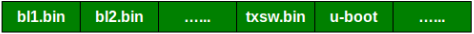
\includegraphics[width=\textwidth]{./data/images/odroid_boot_sequence.eps}
\caption{Odroid Boot Sequence}
\end{figure}

\begin{enumerate}
 \item iROM (Code inside the SoC) will attempt to read the boot media at the first 512 bytes of it. On those first 512 bytes fwbl1 should exist. fwbl1 is signed by Samsung.
 \item fwbl1 will load bl2 (SPL) that is part of the U-Boot. bl2 is signed by Hardkernel
 \item bl2 will load U-boot. U-Boot is signed by us. However, we still have no way to integrate this with the bl2 part.
 \item U-Boot will do whats left, such as handle TrustZone, load kernel image and Ramdisk.
\end{enumerate}

\noindent
\textbf{U-Boot Verified RSA Boot \tobetested{}}

U-Boot has support for booting signed linux kernel images. To enable it we need to define the following variables on U-Boot,

\begin{itemize}
 \item CONFIG\_FIT  enable support for the FIT uImage format
 \item CONFIG\_OF\_CONTROL, CONFIG\_OF\_SEPARATE enable FDT
 \item CONFI\_FIT\_SIGNATURE enables signature verification of FIT images
 \item CONFIG\_RSA enable the RSA algorithm used for FIT image verification
\end{itemize}


and then follow the steps as described at doc/uimage.FIT/* on the U-Boot repository. The kernel will be signed using our custom keys. To boot a signed kernel we need to use the Flat Image Tree (FIT) format provided by U-Boot. This needs to be implemented in a way that does not prohibit us to perform conditional booting (i.e. boot a kernel based on its data integrity; checksum)

\noindent
\textbf{Signed Kernel Modules \tested{}}

The Linux kernel support the signing of modules. This way only modules signed by us would be able to be loaded. See \url{http://wiki.gentoo.org/wiki/Signed_kernel_module_support}



\subsubsection{Application Execution}
\tested{}


The Linux kernel supports the extension of the i-nodes of the file system with hash value of the files and signing of the hash to provide integrity check for files.

In the case that there is a miss match between the stored and the computed hash access is denied to the file.

Linux-IMA (Integrity Measurement Architecture):
\begin{itemize}
 \item \url{http://sourceforge.net/p/linux-ima/wiki/Home/}
 \item \url{https://wiki.gentoo.org/wiki/Integrity_Measurement_Architecture}
 \item \url{http://researcher.watson.ibm.com/researcher/view_group.php?id=2851}
 \item \url{http://lwn.net/Articles/488906/}
 \item \url{http://sourceforge.net/p/linux-ima/wiki/Home/#compiling-the-kernel-with-evmima-appraisal-enabled}
\end{itemize}


IMA-EVM (Extended Verification Module) 
\begin{itemize}
 \item \url{https://wiki.gentoo.org/wiki/Extended_Verification_Module}
\end{itemize}


\subsubsection{Kernel Configuration}
Minimal kernel setup (all unneeded modules should be removed). This can help with preventing someone to attach a foreign unit.

\subsubsection{System Updates}

From the techniques described above we get a locked system that is hard to be altered by an attacker. However, a locked system can become outdated and thus easier to exploit. We need to find a secure way to update our system without compromising its security. 

New kernels should be signed with a constant key as this would reside inside the U-Boot. This may also be the case for the IMA scheme too as we probably do not want to update the sign values on every update.

\subsection{Data Integrity}

All communication is encrypted. Probably use symmetric encryption to reduce overhead.

We need to be able to verify the integrity of the data that are send on the cloud. Otherwise, a compromised control node or guest node can fill the storage with bogus data.

\subsection{Monitoring}

Eagle-eye view of the nodes. Reports on logins, permission denials, changes in important files, attempts of physical break.

See appendix A for monit


\section{Survivability}

Why is survivability required

Expensive to physically access the devices (huge numbers, transportation cost, etc)

\subsubsection{Detection of Improper Shutdown}

Detect improper shutdown of a system so as to run self-check and reconfigure if need be.

This can be implemented through a script that is executed during boot and shutdown. An example for such a scipt, based on the upstart framework, is given below.

\lstinputlisting{./data/improper_shutdown.conf}

\subsection{Redundancy in Kernel Boot Process}

Create conditional booting based on hash checks of binaries.

\subsection{Periodic Check of File System Consistency}

File system consistency needs to be checked periodicly and at specific key steps (before shutdown, during boot). Find hardware problems or file system inconsistent state. Use of journaling file system where possible.

\subsection{Graceful Degradation}
Graceful degradation is an important aspect of survivability. If left unconstrained faulty parts can result in a useless board, whereas, taming and instrumentation can prolong its lifespan and continue of operation until the next maintenance/repair/replace cycle.

\subsubsection{Improper Shutdown Detection}

An improper shutdown can be a sign that the systems resources need to be restricted as they make it unstable.

\begin{itemize}
 \item Crash due to overheating: reduce number of active CPUs
 \item Crash due to power supply problem (IR drop): switch unnecessary modules off
 \item Memory error: isolate memory bank
 \item Kernel crash: disable faulty module
 \item File system error: disable sector
 \item Run out of power: try to improve power usage (coordination of battery and renewable resources)
\end{itemize}




\subsubsection{Reduce number of available CPUs and Memory Nodes}

A part of graceful degradation would be the choice to restrict the number of active (i.e. available for execution) CPUs of the system, or the setting of an upper utilization limit for the processing cores. For this we can use the ``cpuset'' application. See \url{http://man7.org/linux/man-pages/man7/cpuset.7.html}, \url{https://www.kernel.org/doc/Documentation/cgroups/cpusets.txt}, \url{https://www.suse.com/documentation/slerte_11/slerte_tutorial/data/slerte_tutorial.html}, \url{http://techpubs.sgi.com/library/tpl/cgi-bin/getdoc.cgi?coll=linux&db=bks&srch=&fname=/SGI_Admin/LX_Resource_AG/sgi_html/ch01.html} and \url{https://code.google.com/p/cpuset/}

\subsection{System Monitoring}

Logging of system metrics such as utilization, cpu frequency changes, network traffic, logins, etc... can be useful for security, debugging and graceful degradation.

See appendix A for monit. See appendix B for collectl and colmux.

\subsection{Kernel Panic and Module Crash Handling}

Kernel panics are impossible to contain and would certainly result in a system freeze, in such a case the system needs record as much state as possible to help debugging and then force a restart possible using different kernel version. Module crashes are more managable and will not necesarily leave the system hanging, as in the kernel case state needs to be logged and an attempt to clean and reload the module needs to be made. If a reload is impossible and the module serves an important function a full system restart may be used.

\subsection{Application Restart}

In case of crashes important applications need to be restarted. Use of 'monit' or 'systemd'

\section{Power Efficiency}

why and in what degree is power efficiency a requirement

Embedded systems have traditionally been the most power constrained computer systems. For deployment in urban areas these requirement is preserved but can be relaxed as it is easier to provide power on the system. In an urban environment provision can be made so that the system could switch to the town's electic distribution network when its battery or renewable resource are unsaficient. On the other hand, in rural areas power efficiency is much more important due to lack of an extensive power grid.

\subsection{Peripherals}

The choice of peripherals used has an impact on power consumption. As we show different usb-to-ethernet modules where consuming different amount of energy.

\begin{center}
 \begin{tabular}{| l | c |}
 \hline
   & Ampere \\
 \hline
 \hline
 Idle &  \\
 \hline
 + Ethernet1 & \\
 \hline
 + Ethernet2 & \\
 \hline
 + Keyboard & \\
 \hline
 \end{tabular}
\end{center}

Peripherals that are not necessary should be removed from the final deployment package (keyboard, UART)


\subsection{Local vs Remote processing}

In general the following can be assumed for cost of local versus remote processing of data.

\begin{center}
 \begin{tabular}{| l | c | c |}
 \hline
   & Processing Cost & Transfer Cost \\
 \hline
 \hline
 Local Processing & High & Low \\
 \hline
 Remote Processing & Low & High \\
 \hline
 \end{tabular}
\end{center}


A quick and low cost heuristic needs to be created in-order to decide if we will forward or process the raw sensor data.

\begin{lstlisting}
If (local_process_cost + processed_data_transfer_cost > raw_data_transfer_cost) {
  send(raw_data)
} else {
  process(raw_data)
  send(processed_data)
}
\end{lstlisting}

Another consideration especially when wireless communication is used, is the cost of dropped packages or retransmissions. In some cases the cost of retransmissions could surpass the power difference between local and remote processing of data. Thus the above algorithm should be augmented to represent that relation; possibly by multiplying the transfer cost with a retransmission factor.

\noindent
\textbf{Compression}

Use compression to reduce transmission cost. Can be beneficial under constraints.

\noindent
\textbf{Elastic Fidelity Computations}

Sensors are inherently faulty, thus imprecise computation can be employed to improve power efficiency


\subsection{Encryption}

Encryption is a process expensive process thus a power expensive one too. One approach to reduce power consumption of the encryption steps on the framework is to adopt symmetric encryption whenever possible. Also, different libraries could be profiled to find if there are significant benefits on choosing the one over the other.

\subsection{Kernel}

Kernel can be tuned to improve the power efficiency of the device. A first step would be to minimize the number of modules running at any point. Moreover, we can use a governor that has power-saving as a metric.

\textbf{WARNING: kernel 3.8 has a bug that causes reboot to fail when using the powersave governor. Use ``echo performance > /sys/devices/system/cpu/cpu0/cpufreq/scaling\_governor'' before reboot}


\begin{verbatim}
CPU Power Management  --->
 CPU Frequency scaling  --->
  Default CPUFreq governor (performance)  --->
   ( ) performance
   (X) powersave
   ( ) userspace
   ( ) ondemand
   ( ) conservative
\end{verbatim}


\subsection{The Buffer: buffer between the external and internal API}

The buffer in between the internal and external networks can be used to improve power efficiency. By choosing different policies for handling package forwarding we can reduce the consumed power. The reduced power comes at the cost of loss of accuracy.

The policies should be considered a second level techniques as initialy the polling frequency of the sensor should be altered; changing the polling frequency would provide even greater benefits. 

\subsubsection{Policies}

\begin{itemize}
 \item package drop
 \item sampling
 \item averaging
 \item compression
\end{itemize}


\appendix

\section{mkcard}
\label{appendix:mkcard}

\lstinputlisting{scripts/mkcardOdroid.sh}

\section{cpuset}
\label{appendix:cpuset}

information regarding cpuset. cpusets: what do they support, what are the limitations, what do we need to change to overcome them.



\bibliography{main}{}
\bibliographystyle{plain}

\end{document}
